In recent times, the need to store more and more information increased 
a lot thanks most of all to machine-generated data: we will understand how
we store all our data and what to use based on the purposes of said data
and the machine that uses them. We know mainly 4 types of memories:
\begin{itemize}
    \item HDDs - Magnetic disks with mecanical action, currently dominating
    the storage technology
    \item SSDs - Faster and without mechanical parts, transistor-only
    \item NVMe - Non Volatile Memory express, for PCle SSDs
    \item Tapes - \textbf{will never die} (see S3 Glacier Data Center)
\end{itemize}
Combinations of memory types are possible (like SSHD, where a small SSD is
combined with a main HDD) and also NVDIMM (Non-Volatile Dual In-Line Memory
 Module, a solution to keep data when power goes out and with the same speed 
 of a DRAM).
 \begin{notice}{We trash the majority of what we produce!}
    We discovered that it is way cheaper to acquire data than 
    to store it: this means that the majority of the produced data gets 
    thrown away or gets elaborated in real-time tasks. Actually, the 
    \textbf{network} is the most stressed components, since lots of data 
    that never gets stored passes through there.
    \begin{figure}[H]
        \centering
        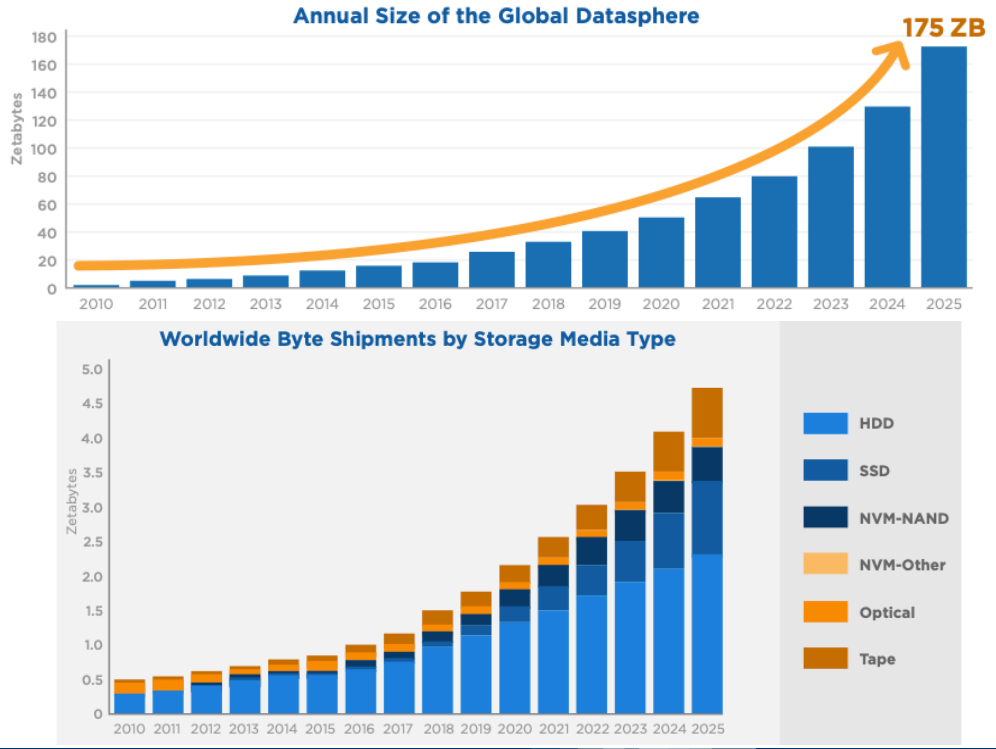
\includegraphics[width=1\textwidth]{Images/15Data.png}
        \caption{Real world data}
    \end{figure}
 \end{notice}
 \subsection{HDD}
 \subsubsection{Quick summary on the basis of a file system}
 \begin{itemize}
    \item Disks can be seen by an OS as a collection of \textbf{data blocks}
    \item Each data blocks has an address called 
    \textbf{Logical Block Address}
    \item Blocks are usually grouped into \textbf{clusters}, the minimal unit
    that a OS can read, and are measured in \textbf{sectors} 
    (1 sector = 512B)
    \item Clusters contain \textbf{file data} and \textbf{meta data}(file 
    names, directory structures, etc) 
\end{itemize}
\begin{figure}[H]
    \centering
    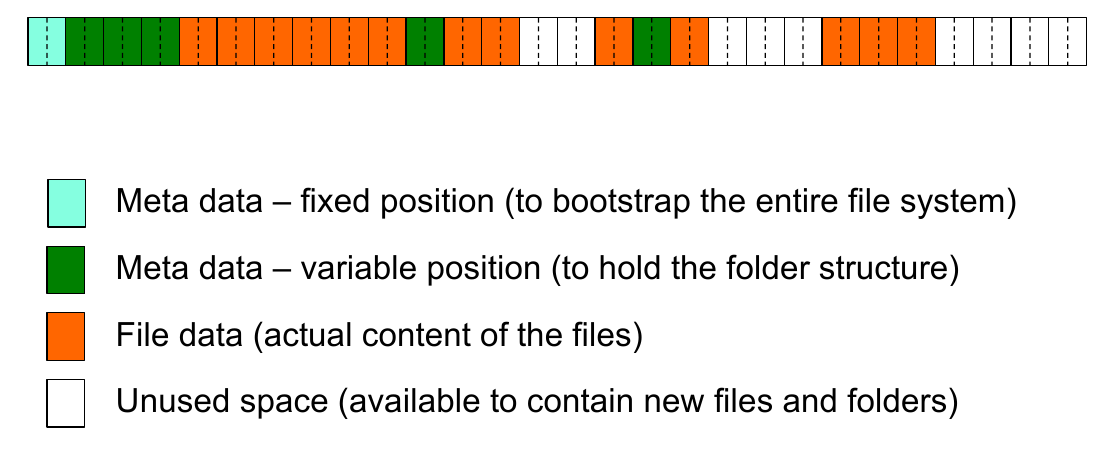
\includegraphics[width=1\textwidth]{Images/16FileSystem.png}
    \caption{Example of FS}
\end{figure}
\begin{itemize}
    \item A typical file read operation requires to read meta data and then to 
    access the real data, a typical write operation requires to read meta data
    to locate empty space and then to write in the right address
    \item Wasted disk space is generated due to the organization of the file 
    structured into clusters
    \item The deletion of file data is the \textbf{unlinking} of the meta data 
    associated with said file, not the deletion of the files themselves: that's
    because data never gets deleted on disk, but only \textbf{overwritten}
    \item When a file is too big to be stored contiguously i use 
    \textbf{external fragmentation} to store pieces of the file in a 
    non-contiguous way: this is the main flaw of HDDs
\end{itemize}
\begin{key}{HDDs}
    A Hard Disk Drive is a data storage device that uses rotating disks to 
    read and write informations: the action of accessing data is random, not
    sequential as in tapes.
\end{key}
Individual sector writes are \textbf{atomic} operations, also:
\begin{itemize}
    \item Sectors are arranged into \textbf{tracks}
    \item A \textbf{cylinder} is a particular track on multiple platters
    \item Tracks are arranged in \textbf{concentric circles} on platters
    \item A disk may have multiple, double-sided platters
    \item Drive motor spins the platters at a constant rate 
    measured in revolutions per minute (\textbf{RPM})
\end{itemize}

\begin{figure}[H]
    \centering
    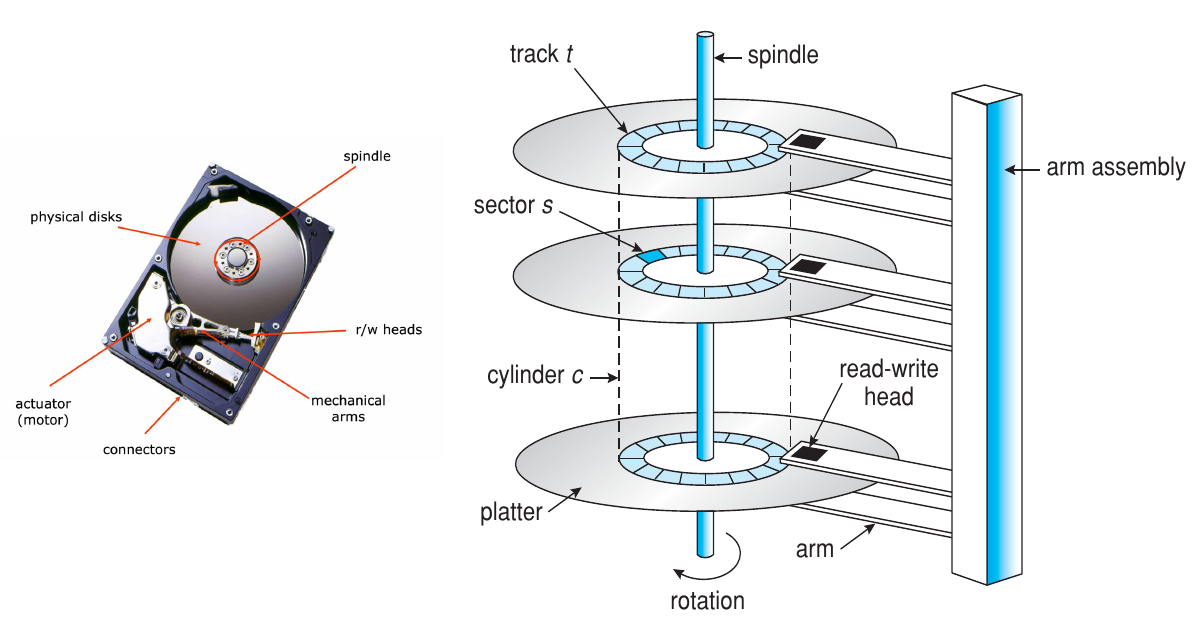
\includegraphics[width=1\textwidth]{Images/17HDDs.png}
    \caption{HDDs exploded}
\end{figure}
HDDs have lots of possible delays:
\begin{itemize}
    \item \textbf{Rotational Delay} - the time to rotate the desired sector 
    to the head
    \item \textbf{Seek Delay} - the time to move the read head to a different 
    track
    \item \textbf{Transfer Time} - the time to read or write bytes
    \item \textbf{Controller Overhead} - the time used for the request 
    management
\end{itemize}

\subsubsection{All Delays}
\begin{formula}{Rotation Delay}
    Defining $R$ as the full rotation delay in $1/\text{DiskRPM}$,
    \begin{equation}
        \begin{aligned}
            T_{\text{AvgRotation}} = 60 * R
        \end{aligned}
    \end{equation}
\end{formula}

\begin{formula}{Seek Delay}
    Seek delay follows an idealized \textbf{linear model}, with direct 
    dependence on the distance of access.
    \begin{figure}[H]
        \centering
        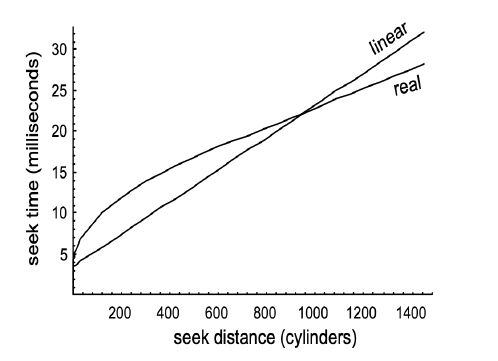
\includegraphics[width=0.5\textwidth]{Images/18SeekTime.png}
        \caption{Reality vs linear idealization}
    \end{figure}

    We can define an average seek time as:
    \begin{equation}
        T_{\text{AvgSeek}} = T_{\text{MaxSeek}} / 3
    \end{equation}
\end{formula}

\begin{formula}{Transfer and Control Delay}
    Those delays are considering the time that is wasted during direct 
    read/write operations.
\end{formula}
\begin{formula}{Service Time}
    The service time of an operation is the full time that passes from its 
    start and completion.
    \begin{equation}
        \begin{aligned}
            T_{I/O} = T_{\text{Seek}} + T_{\text{Rotation}} + 
            T_{\text{Transfer}} + T_{\text{Overhead}}
        \end{aligned}
    \end{equation}
\end{formula}

\begin{ex}
    Let's analyze the read/write operation of a sector of 512B (= 0.5KB).
    Having:
    \begin{itemize}
        \item a data transfer rate = 50MB/s
        \item a rotation speed = 10000 RPM
        \item a mean seek time = 6ms
        \item an overhead controller = 0.2ms
    \end{itemize}
    What is the \textbf{total service time}? \newline
    We know the general equation to calculate the $T_{I/O}$, we can see that 
    $T_{\text{Seek}} = 6ms$ but we need to calculate the true rotation time:
    \begin{equation}
        T_{Rotation} = \frac{60s/min * 1000}{2 * 10000 \text{RPM}} = 3\text{ms}   
    \end{equation}
    This time is calculated for half round. We can then calculate the transfer 
    time as
    \begin{equation}
        T_{\text{Transfer}} = \frac{0.5KB * 1000}{50 * 1024KB/s} = 0.01\text{ms}    
    \end{equation}
    Finally, we compute the total time:
    \begin{equation}
        T_{I/O} = 9.21ms   
    \end{equation}
    Remember: this is a \textbf{pessimistic example}, the mechanical latency
    is payed every time we "jump" from a sector to another: not always this 
    is done in a read/write operation. You can see in the slides another 
    two examples where it is considered the vaule of \textbf{data locality}.
\end{ex}

\subsubsection{Caching and Scheduling}
Many disks implement small caches of 8, 16 or 32MB for reduced time wasted on 
read operations and also in writing:
\begin{itemize}
    \item \textbf{Write Back Cache} - drive reports that writes are complete
    after they have been cached
    \item \textbf{Write Through Cache} - drive reports that writes are complete
    after they have been written to disk
\end{itemize}
This helps to improve performance but it cannot make up for poor random
access: \textbf{disk schedulers} on the other hand help to decide what
disk operation do in what order, so that "near sector" operations can be 
done close to each other to avoid wasting time into mechanical movement.
Many scheduling policies can be used:
\begin{itemize}
    \item \textbf{FCFS} (First Come First Served) - requests are served in order
    \item \textbf{SSTF} (Shortest Seek Time First) - requests are served based
    on the closest seek time address (evalued after every request), easy to 
    implement and gives good results but there may be \textbf{starvation}
    \item \textbf{SCAN} - requests are served by scanning the whole disk
    addresses: worse performance than than SSTF, but better for fairness
    \item \textbf{C-SCAN} (Circular SCAN) - requests are served in a one-sweep
    direction
    \item \textbf{C-LOOK} - identical to C-SCAN but the sweep goes not from 
    edge-to-edge of disk space, they reach the farthest request
\end{itemize}

\begin{notice}{Where should the scheduler be?}
    Actually it depends, there are different solutions around:
    \begin{itemize}
        \item OS Scheduling
        \item On-Disk Scheduling
        \item Disk Command Queue
    \end{itemize}
    (see slides)
\end{notice}

\subsection{SSD}
SSD are solid state storage devices with no mechanical parts built out of
transistors: they retain informations despite power loss and offer higher
performances than HDD. Data is stored in cells, there are various ways to 
store informations inside: \textbf{SLC} (a single bit per cell), \textbf{MLC}
(two bits per cell), \textbf{TLC}, \textbf{QLC},...
\begin{figure}[H]
    \centering
    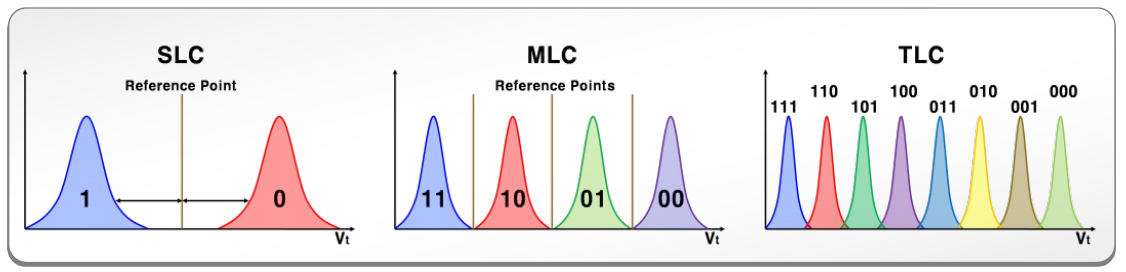
\includegraphics[width=1\textwidth]{Images/19Cells.png}
    \caption{Different Cell Organizations}
\end{figure}
The problem in storing multiple bits in a single cell is that to identify said
sequence of bits i need to assign them \textbf{different voltage levels}: this
means that if i want to read the value of a cell i need to \textbf{wait} for 
the transient to pass through (maybe) the full value of the maximum voltage.
\begin{notice}{Smaller is Faster}
    That's why SLC are faster than MLC!
\end{notice}
NAND flash is organized in pages (that contains multiple logical blocks) and
blocks that contains multiple pages (don't mess up with previous general
data definitions: this is only SSD related!): a block is considered by the 
SSD as the smallest unit of information stored when deleting, this means that 
when erasing a block we are actually erasing multiple pages. On the other hand,
pages are the smallest unit that can be read or written: pages can be marked 
as \textbf{erased}, \textbf{dirty} (invalid data) or \textbf{valid}.

\subsubsection{Performance Issues}
The main problem of SSD is that "in theory" it is fast and reliable, but 
in real circumstances the fact that they have a big mismatch with HDD systems
in terms of usage gives way to a lot of issues: the main mismatch being that 
\textbf{SSD reads pages but deletes whole blocks} and that \textbf{a page can
be marked in three different ways}. Let's see an example with a made up SSD
memory block of 5 pages.
\begin{figure}[H]
    \centering
    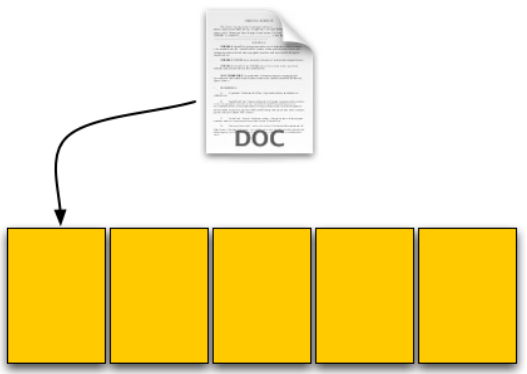
\includegraphics[width=0.4\textwidth]{Images/20Blocks1.png}
\end{figure}
If i wanted to save a document of 4KB of space and my write speed is of 
1KB/s then i would spend 4s of time to save said file.
\begin{figure}[H]
    \centering
    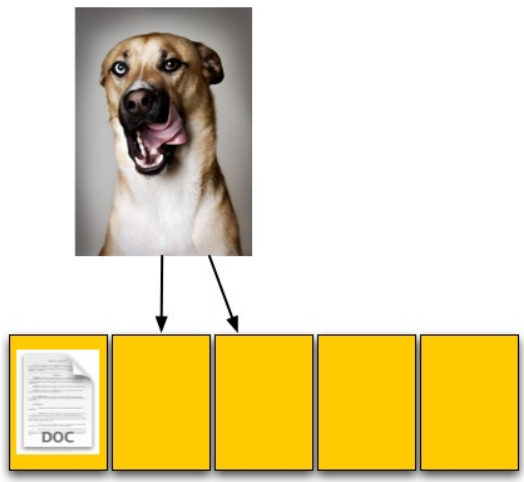
\includegraphics[width=0.4\textwidth]{Images/21Blocks2.png}
\end{figure}
Again, with a bigger file no problems in saving it since there's space that can
be used.
\begin{figure}[H]
    \centering
    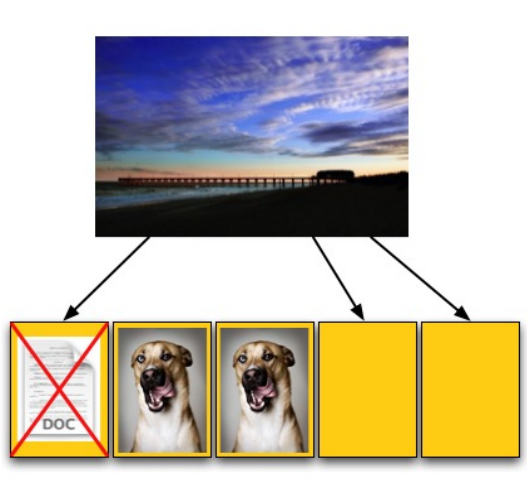
\includegraphics[width=0.4\textwidth]{Images/22Blocks3.png}
\end{figure}
Real problems start when i decide to delete the document that i wanted to save 
and then try to put a new, bigger file that now needs all the remaining block's 
space: since i can only delete \textbf{whole blocks} and not single pages i 
forcely need to save all the files temporally inside a cached space, delete 
the "dirty" document that i wanted to delete inside the cache, add the new 
image inside the cache, delete the whole block of memory inside the SSD and 
then write the cache into the SSD. Instead of having 12s of delay i had 24s. 
\newline
This problem is known as the \textbf{write amplification effect}.

\subsubsection{Flash Transition Layer}
Also, since direct mapping between logical and physical pages is not feasible,
the SSD memory needs to have a component called \textbf{FTL} that makes the SSD
look like an HDD: it comes with \textbf{data allocation and address translation}
(useful to prevent write amplification effects), \textbf{garbage collection}
(to better reuse pages with old data) and \textbf{wear leveling} (SSD wears
overtime, it's a technology with a known obsolescence limit).
